\documentclass[10pt,a4paper]{article}


\newenvironment{changemargin}[2]{%
\begin{list}{}{%
\setlength{\topsep}{0pt}%
\setlength{\leftmargin}{#1}%
\setlength{\rightmargin}{#2}%
\setlength{\listparindent}{\parindent}%
\setlength{\itemindent}{\parindent}%
\setlength{\parsep}{\parskip}%
}%
\item[]}{\end{list}}

\usepackage[latin1]{inputenc}
\usepackage{amsmath}
\usepackage{amsfonts}
\usepackage{amssymb}
\usepackage{listings}
\usepackage{graphicx}
\title{Assignment No :A3}
\date{}


\begin{document}
\maketitle
\section{Title:}
Booth's multiplication

\section{Problem Definition}
A Web Tool for Booth's multiplication algorithm is used to multiply two numbers located in distributed
environment. Use software design client-server architecture and principles for dynamic programming.
Perform Risk Analysis. Implement the design using HTML-5/Scala/ Python/Java/C++/ Rubi on Rails.
Perform Positive and Negative testing. Use latest open source software modeling, Designing and testing
tool/Scrum-it/KADOS and Camel.

\section{Learning Objectives}
\begin{enumerate}
\item To understand Booth's multiplication algorithm.
\item To understand binary multiplication.
\item To perform problem analysis using the open source tools.
\end{enumerate}

\section{Learning Outcomes}
\begin{enumerate}
\item Ability to analyze problems as multiplication.
\item Acquired understanding of problem solving using divide and conquer strategies and inducing appropriate parallelism in them.
\item Acquired knowledge about the documentation of typical software programs.
\end{enumerate}


\section{Related Mathematics}
Let S be the solution perspective of the given problem.\\
The set S is defined as:\\\\
$S=\lbrace\ s,e,X,Y,F,DD,NDD,S_{c},F_{c}|\varnothing_{s}\rbrace$ \\
Where,

s= Start state,  Such that $Y=\lbrace \varnothing \rbrace$ 

e= End state  \\\\
X= Input Set. \\\\
$X=\lbrace$ x = $\lbrace x_1, x_2 \rbrace$ $\mid$ x $\in$ NN (natural numbers) $\rbrace$ \\
Where,

NN $\in \lbrace$ Positive Integers $\rbrace$ - 0\\\\ 
Y=Output set.\\
$Y=\lbrace$ $x_1 * x_2$ $\rbrace $ \\\\
F= Set of functions used.\\
F=$\lbrace binarize(), add(), shift(), multiply() \rbrace$ \\\\
binarize() = function to convert the decimal numbers to binary\\
shift() = function to shift a binary number\\
multiply() = the booth's multiplication funciton that multiples two numbers using booth's algorithm and internally makes use of the shift and add functions\\
add() = function to add two binary numbers\\\\
DD=Deterministic data. \\
DD=
\begin{enumerate}
\item input numbers are proper (no hardware overflow).
\item numbers are natural numberes.
\item multiplication terminates (the numbers are finite)\\\\
\end{enumerate}
NDD= Non-deterministic data. \\
\\NDD= $\cup$ - DD\\


\section{State Transition diagram}
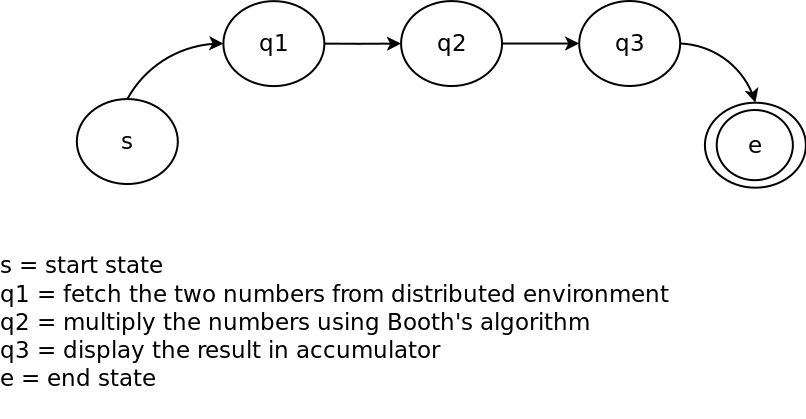
\includegraphics[scale=0.28]{stdg.png}


\section{Concepts related theory}
\subsection{Client server model}
	\paragraph{} The Client-server characteristic describes the relationship of cooperating programs in an application. The server component provides a function or service to one or many clients, which initiate requests for such services.
	\paragraph{}Servers are classified by the services they provide. For instance, a web server serves web pages and a file server serves computer files. A shared resource may be any of the server computer's software and electronic components, from programs and data to processors and storage devices. The sharing of resources of a server constitute a service.
	\paragraph{} Whether a computer is a client, a server, or both, is determined by the nature of the application that requires the service functions. For example, a single computer can run web server and file server software at the same time to serve different data to clients making different kinds of requests. Client software can also communicate with server software within the same computer.Communication between servers, such as to synchronize data, is sometimes called inter-server or server-to-server communication.
		
		\begin{figure}[htb!]
			\centering
			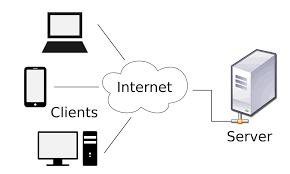
\includegraphics{images.png}
			\caption{Client Server Model}
			\label{Client Server Model}
		\end{figure}
		
\subsection{Client Server Communication:}
	\paragraph{} In general, a service is an abstraction of computer resources and a client does not have to be concerned with how the server performs while fulfilling the request and delivering the response. The client only has to understand the response based on the well-known application protocol, i.e. the content and the formatting of the data for the requested service.
	\paragraph{} Clients and servers exchange messages in a request - response messaging pattern: The client sends a request, and the server returns a response. This exchange of messages is an example of inter-process communication. To communicate, the computers must have a common language, and they must follow rules so that both the client and the server know what to expect. The language and rules of communication are defined in a communications protocol. All client-server protocols operate in the application layer. The application-layer protocol defines the basic patterns of the dialogue. To formalize the data exchange even further, the server may implement an API (such as a web service). The API is an abstraction layer for such resources as databases and custom software. By restricting communication to a specific content format, it facilitates parsing. By abstracting access, it facilitates cross-platform data exchange.
	\paragraph{} A server may receive requests from many different clients in a very short period of time. Because the computer can perform a limited number of tasks at any moment, it relies on a scheduling system to prioritize incoming requests from clients in order to accommodate them all in turn. To prevent abuse and maximize uptime, the server's software limits how a client can use the server's resources. Even so, a server is not immune from abuse. 



\subsection{Booth's Algorithm flow chart}
	\begin{figure}[h!]
		\centering
		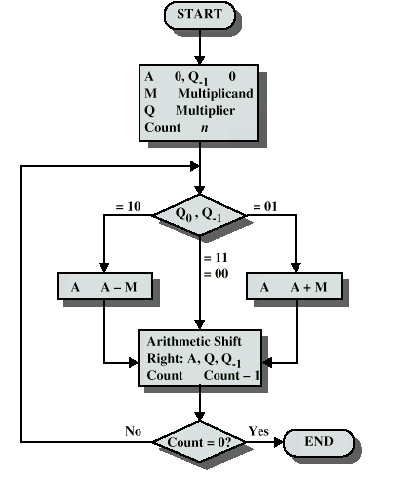
\includegraphics[scale=0.60]{booth}
		\caption{Booth's Multiplication Flowchart}
	\end{figure}

	\begin{figure}[htb]
		\centering
		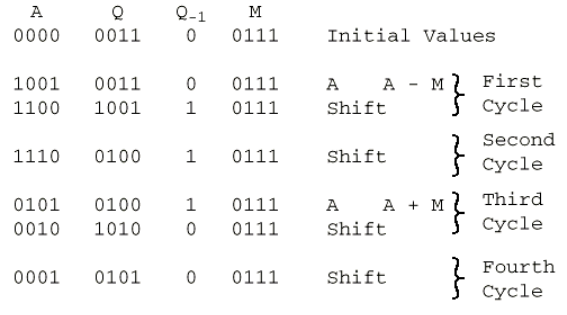
\includegraphics[scale = 0.60]{boothex}
		\caption{ Multiplication (7*3) using Booths Algorithm}
	\end{figure}

\newpage
\section{Object oriented modelling}
\subsection{Use Case Diagram}
	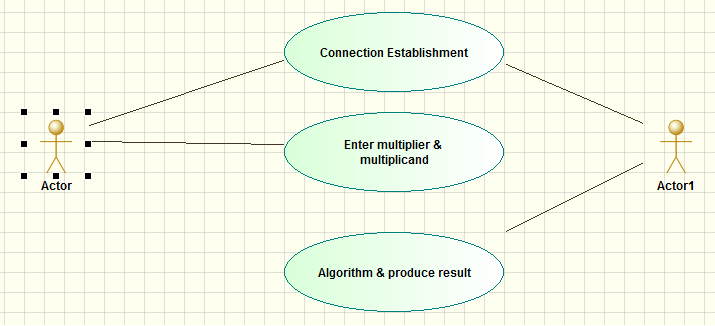
\includegraphics[scale=0.8]{usecase}


\subsection{Activity Diagram}
	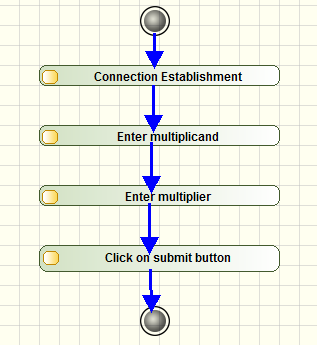
\includegraphics[scale=0.95]{activity}
			
\subsection{Class Diagram}
	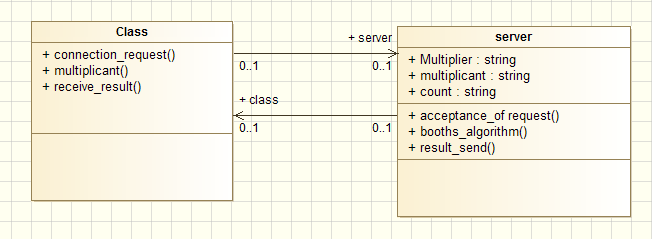
\includegraphics[scale=0.95]{class}

\newpage
\begin{changemargin}{-4cm}{-4cm}
\section{Program Listing}
\begin{lstlisting}

# BitFieldsOperations.py

'''
	This library keeps the implementations of some of 
the binary oprations frequently performed on the 
bitfields

	*****************************************************
	**** The main assumption for this library to work 
	**** properly is that the bitfield lengths are 	
	**** already nibble
	**** size optimised. Some functions may work 
	**** properly, but most may fail. So, make sure 	
	**** they are in the required format	
	******************************************************
'''


# as suggested by (@Murtaza Raja view --> https://github.com/murtraja) :)
def bitLenEqualize(num1, num2):
	'''
		method to equalize the number of bits in both numbers
			
		@params
		num1 = the bitfield for the restricted number 1
		num2 = the bitfield for the restricted number 2
	'''
	sign1 = num1[0]; sign2 = num2[0] # extract the sign bits of the two numbers
	
	# unset the two bits for both the numbers
	num1[0] = 0
	num2[0] = 0 
	
	# pad the number with lesser length to be equal to the onther one
	while(len(num1) != len(num2)):
		if(len(num1) < len(num2)):
			# add a nibble to the first number
			num1 = [0 for i in range(4)] + num1

		else: 
			# add a nibble to the second number
			num2 = [0 for i in range(4)] + num2

	# before returning the bitfields, retrun their origingal sign bits back to them
	num1[0] = sign1
	num2[0] = sign2

	return num1[:], num2[:]

def rsa(num, times):
	'''
		method to perform the arithmetic right shift on the binary number
			
		@params
		num = the bitfield for the restricted number
		times = number of times the shifting needs to be performed
	'''
	assert (times > 0), "you cannot shift a number -ve number of times"

	for i in range(times):	# perform the shift times number of times
		num.pop(len(num) - 1) # remove the last element of the bitfield
		num = [num[0]] + num
		
	return num[:]



def rsc(num, times):
	'''
		method to perform the circular right shift on the binary number
			
		@params
		num = the bitfield for the restricted number
		times = number of times the shifting needs to be performed

		@return
		a bitfield of the multiplication of the two numbers
	'''
	assert(times > 0), "you cannot shift a number -ve number of times"
	
	for i in range(times):
		bit = num.pop(len(num) - 1) # remove the last element of the bitfield
		num = [bit] + num
		
	return num[:]



def add(n1, n2):
	'''
		method to add the bitfields of two binary numbers
		*** Truncates the final carry by default ***			

		@params
		n1 = the bitfield for the restricted number1
		n2 = the bitfield for the restricted number2

		**** Implementation can be improved ****
	'''	

	# use the bitLenEqualize function to equalize the number of bits of the two numbers
	n1, n2 = bitLenEqualize(n1[:], n2[:]) 

	# carry on with the addition part
	bsum = [0 for i in range(len(n1))]; carry = 0		
			
	for i in reversed(range(len(n1))): 
		# a complete hardwired implementation of binary addition
		if(n1[i] == 0 and n2[i] == 0): 
			if(carry == 0): 
				bsum[i] = 0	
			else: 
				bsum[i] = 1
				carry = 0

		elif(n1[i] == 0 and n2[i] == 1):
			if(carry == 0): 
				bsum[i] = 1	
			else: 
				bsum[i] = 0
		 				
		elif(n1[i] == 1 and n2[i] == 0): 
			if(carry == 0): 
				bsum[i] = 1	
			else: 
				bsum[i] = 0
		
		elif(n1[i] == 1 and n2[i] == 1): 
			if(carry == 0): 
				bsum[i] = 0
				carry = 1	
			else: 
				bsum[i] = 1
			
	return bsum[:]



def t2scomp(num): 
	'''
		method to calculate the 2's complement of the binary number
			
		@params
		num = the bitfield for the restricted number
	'''
	for i in range(len(num)): # flip every bit of the input number
		if(num[i] == 1):
			num[i] = 0
		else:
			num[i] = 1
				
	return add(num[:], ([0 for i in range(len(num) - 1)] + [1])[:]) # add 1 and return



# BoothMultiplier.py
from BitFieldsOperations import * # the library created by botman present in the same package


''' The following error handler function is no longer required as there are no more assertion errors being thrown from the code below'''
# error handler function for AssertionError types of errors
#def handleAssertionError():
#	'''
#		Helper method for the api to be used to handle the various types of assertion errors that might be thrown
#	'''
#	_, _, tb = sys.exc_info()
#	tb_info = traceback.extract_tb(tb)
#	filename, line, func, text = tb_info[-1]
#	error = text.split(",")[-1]
#
#	print "An error occured: " + error



class BitNibbles:
	'''
		The class that converts a number into binary and stores the bits in its object
	'''

	def __convert_to_binary(self, number):
		'''
			Private helper method to convert the given integer into list of bits
		'''

		bits = [int(digit) for digit in bin(abs(number))[2:]] # get the list of bits

		# nibble size optimisation of the bitfield
		while(len(bits) % 4 != 0):
			bits = [0] + bits # add a 0 in the front

		# if the first bit is 1, we have to still add 4 more 0s
		if(bits[0] == 1):
			bits = [0 for i in range(4)] + bits

		# if the number is negative, represent it in the 2's complement form
		if(number < 0):
			bits = t2scomp(bits[:])

		return bits


	def __init__(self, integer): # default size of limit is 8 bits
		'''
			Default constructor of the class.

			@params
			integer = the number that needs to be converted to bits
			limit  	= size of the binary number in bits. by default it is 8 bits i.e. 2 nibbles
		'''

		# convert the number from decimal to a binary bitfield
		bitfield = self.__convert_to_binary(integer)

		# private data attributes
		self.__size = len(bitfield) // 4 # a reference to the current size of the bitfield in number of nibbles
		self.__bits = bitfield # assign the bitfield to the bits



	def getBits(self):
		'''
			getter method to acquire the converted bits.
		'''

		return self.__bits[:] # to return the value and not the reference to the list

	def getSize(self):
		'''
			getter method to acquire the set size of the number.
		'''

		return self.__size # to return the value and not the reference to the list



class BoothMultiplier:
	'''
		Algorithm class to encapsulate the booth's algorithm multiplier
	'''

	@staticmethod
	def multiply(num1, num2):
		'''
			Multiply two numbers using the Booth's binary multiplication algorithm

			@params
			num1  =  the BitNibbles object representing the number 1
			num2  =  the BitNibbles object representing the number 2
		'''
		# extract the bits for the two numbers
		bits1 = num1.getBits()
		bits2 = num2.getBits()

		# equalize the lengths of the bitfields for the two numbers
		bits1, bits2 = bitLenEqualize(bits1[:], bits2[:])


		# verbose log statements for the console
		print "\n\nThe multiplication is to be carried out between: "
		print "No. 1: ", bits1
		print "No. 2: ", bits2


		# The actual algorithm starts from here:
		# some more comments added for readability

		# refer the video link -> https://www.youtube.com/watch?v=1aTR9WQFFtM
		# for more information. I have used the same names for the variables used in the video.

		# the uv array keeps the final answer
		uv = [0 for i in range(2 * len(bits1))] # initialize the uv array to all 0s


		# number 1 for the multiplication (multiplicand)
		x = bits1[:] # just renaming it for simplicity's sake (as used in the video)


		# number 2 for the multiplication (multiplier)
		y = bits2[:] + [0 for i in range(len(bits2))] # again name changed and size adjusted
		# although, the add function now adjusts the size, I have still kept it like this


		# the -ve of the the second number that needs to be added in some cases
		_y = t2scomp(bits2[:]) + [0 for i in range(len(bits2))] # basically, the -y value

		# the (x - 1) bit required for the algorithm.
		x_1 = 0 # always initialized to 0


		# start the loop for the algorithm
		for i in range(len(x)):

			# if the last bit of x is 0 and (x-1) bit is 1, take this action
			if(x[-1] == 0 and x_1 == 1):
				# case when y value is to be added to the answer (uv)
				uv = add(uv[:], y[:])

			# if the last bit of x is 1 and (x-1) bit is 0, take this action
			elif(x[-1] == 1 and x_1 == 0): # this cannot be simple else, because there are two more cases (0, 0) and (1, 1)
				# case when y value is to be subtracted (add 2's complement of the y value)
				uv = add(uv[:], _y[:])


			# in every case, this has to be always performed

			# arithmetic right shift uv array by 1
			uv = rsa(uv[:], 1)

			# update the x - 1 value
			x_1 = x[-1]

			# circular right shift the x value by 1
			x = rsc(x[:], 1)

			# verbose log statements
			print "Current Step: ", i + 1
			print uv, "\n"

		# verbose log statements
		print "Answer of Multiplication: ", uv
		return uv
		

# Runner.py

'''
    The UI runner script for the Booth's Multiplication Api.
    *******************************************************
    ** @required
    ** 1.) python2.7
    ** 2.) Bottle framework
    *******************************************************
    *******************************************************

    #codedByBotman
'''

from bottle import Bottle, run, template, request, static_file
from Models.BusinessLogic.BoothMultiplier import * # The botman's api for Booth Multiplication

botApp = Bottle() # create a bottle application object to run the application

# static route to serve the js and css files
@botApp.route('/static/:path#.+#', name='static')
def static(path):
    return static_file(path, root='static')

# default route to land in when the application is started
@botApp.get('/')
def shower():
    return template("home")

# The route that serves the actual multiply request.
@botApp.get('/multiply')
def boothM():
    num1 = int(request.params['num1'])
    num2 = int(request.params['num2'])

    return template("home",
        ans = reduce(
                lambda x, y: x + y, # the reduction function to be applied
                map(str, BoothMultiplier.multiply(BitNibbles(num1), BitNibbles(num2)))
        )
    )

# run the application on localhost and port
run(botApp, # the application that is to be run
    host = "localhost", # the host for the application
    port = 6969 # the port number on which the application will run
)

# home.tpl

<!DOCTYPE html>
<html>
  <head>
    <title> BotMan's BoothMultiplier </title>

    <!-- The beautifying framework files  -->
    <link rel="stylesheet" href="static/css/bootstrap.min.css">
    <script src="static/js/jquery-3.0.0.min.js" charset="utf-8"></script>
    <script src="static/js/bootstrap.min.js" charset="utf-8"></script>

    <!-- This is required to make the page responsive for mobile devices -->
    <meta name="viewport" content="width=device-width, initial-scale=1.0">

  </head>

  <body>
    <header class="jumbotron text-center"
            style="background-color: #00695C; color: white;">
      <h1> <b> Booth Multiplier </b> </h1>
    </header>

    <main>
      <div class="container">
        % include("MultiplyNumbersForm")

        % if(defined("ans")):
          % include("ResultDisplay", answer=ans)
        % else:
          % pass
      </div>
    </main>

  </body>
</html>

# MultiplyNumbersForm.tpl

<div class="panel panel-default">
  <div class="panel-body">
    <div class="col-sm-offset-3 col-sm-8">
      <form action="/multiply" class="form-horizontal" method="get">
        <div class="form-group">
          <label for="multiplicand" class="col-sm-2 control-label"> Num 1: </label>
          <div class="col-sm-6">
            <input type="number" class="form-control" id="multiplicand"
                name="num1" placeholder="Enter a number" required>
          </div>
        </div>
        <div class="form-group">
          <label for="multiplier" class="col-sm-2 control-label"> Num 2: </label>
          <div class="col-sm-6">
            <input type="number" class="form-control" id="multiplier"
                name="num2" placeholder="Enter a number" required>
          </div>
        </div>
        <div class="form-group">
          <div class="col-sm-offset-4 col-sm-10">
            <button type="submit" class="btn btn-success"> Multiply </button>
          </div>
        </div>
      </form>
    </div>
  </div>
</div>

# ResultDisplay.tpl

<div class="panel panel-default">
  <div class="panel-body text-center">
    <h1> Answer = {{ answer }}</h1>

    <div class="alert alert-warning col-sm-offset-4 col-sm-4">
      <h4> <b> Please See the console for more information </b> </h4>
    </div>
  </div>
</div>

\end{lstlisting}
\end{changemargin}


\section{Output}
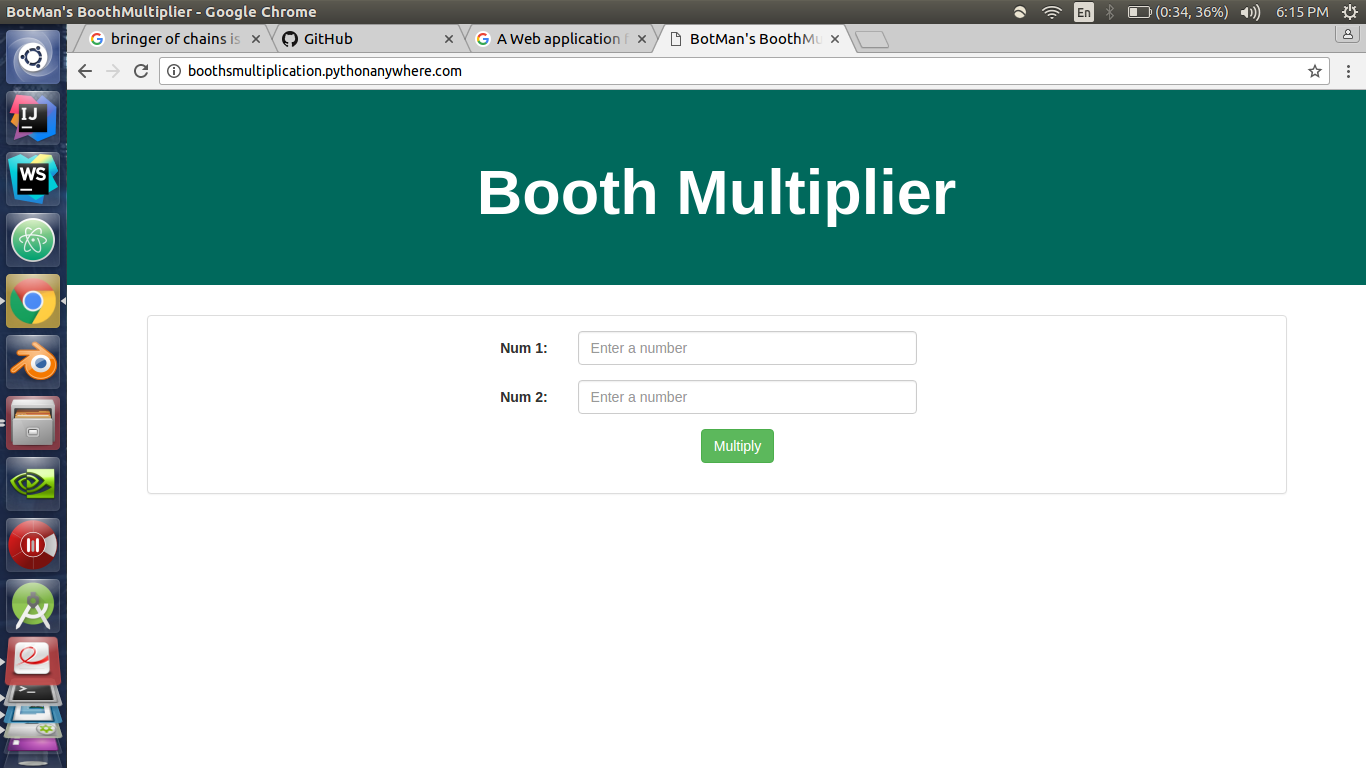
\includegraphics[scale=0.3]{out_1.png}
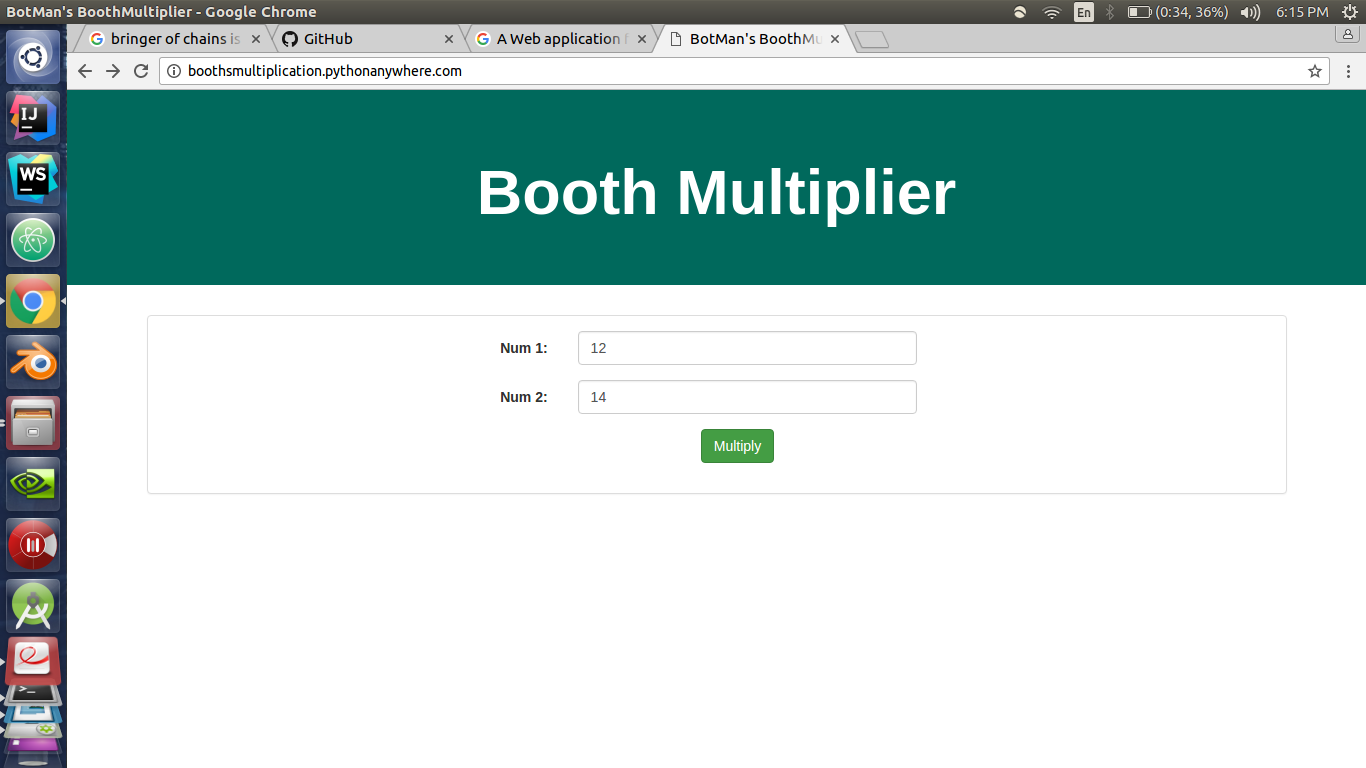
\includegraphics[scale=0.3]{out_2.png}
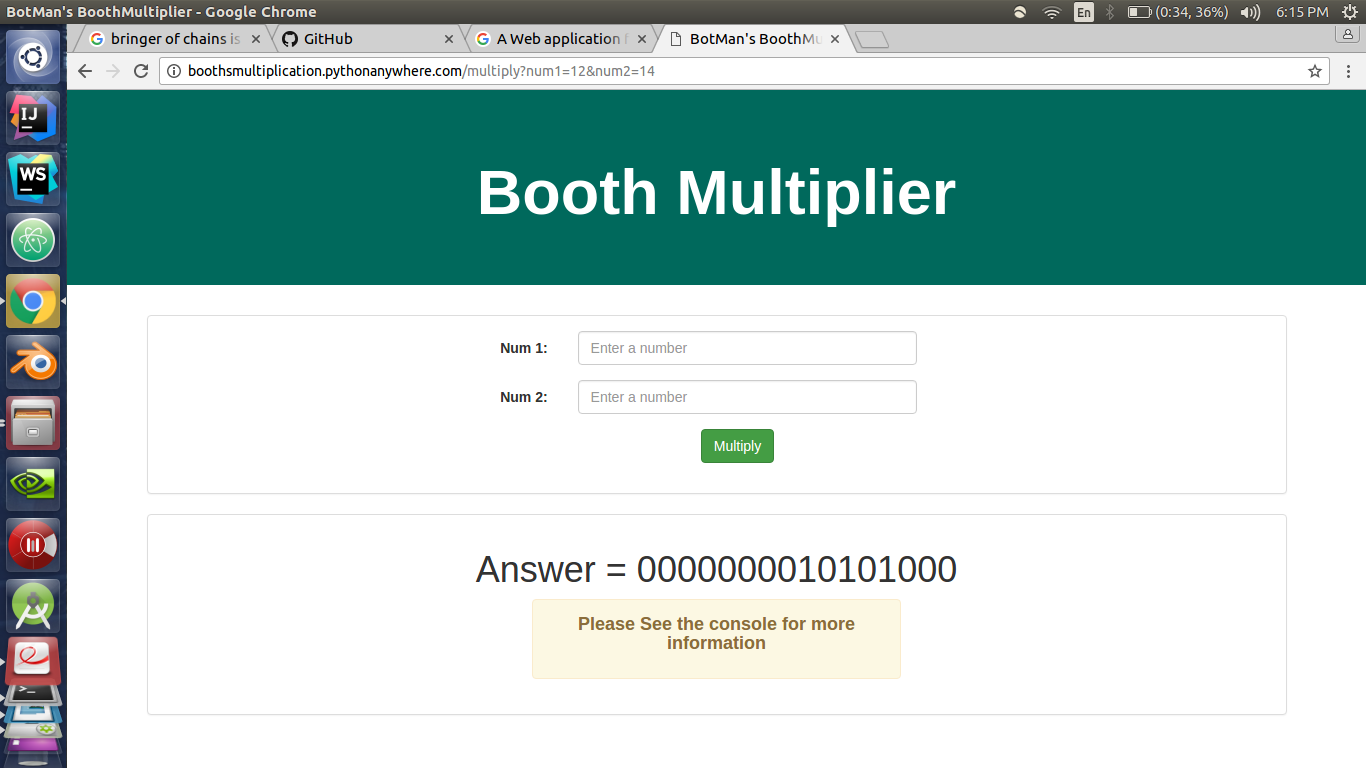
\includegraphics[scale=0.3]{out_3.png}

\section{Testing}
\subsection{BLACK BOX TESTING : }
		 Black-box testing is a method of software testing that examines the functionality of an application based on the specifications. It is also known as Specifications based testing. Independent Testing Team usually performs this type of testing during the software testing life cycle.This method of test can be applied to each and every level of software testing such as unit, integration, system and acceptance testing.\\
		 Black box testing techniques are :\\
1) Equivalence Class Partitioning\\
2) Boundary Value Analysis\\
3) Decision Tables\\
4) State Transition Diagrams (or) State Transition Diagrams\\
5) Orthogonal Arrays\\
6) All Pairs Technique\\

\subsection{WHITE BOX TESTING :}
		 White Box Testing (WBT) is also known as Code-Based Testing or Structural Testing. White box testing is the software testing method in which internal structure is being known to tester who is going to test the software.In this method of testing the testcases are calculated based on analysis internal structure of the system based on Code coverage, branches coverage, paths coverage, condition Coverage etc. Typically such method are used at Unit Testing of the code but this different as Unit testing done by the developer \& White Box Testing done by the testers, this is learning the part of the code \& finding out the weakness in the software program under test.
For tester to test the software application under test is like a white/transparent box where the inside of the box is clearly seen to the tester (as tester is aware/access of the internal structure of the code), so this method is called as White Box Testing.

The White-box testing is one of the best method to find out the errors in the software application in early stage of software development life cycle. In this process the deriving the test cases is most important part. The test case design strategy include such that all lines of the source code will be executed at least once or all available functions are executed to complete 100 percent  code coverage of testing. For this, we will use Flow Graphs. Flow graphs are, Syntactic abstraction of source code Resembling to classical flow charts Forms the basis for white box test case generation principles.Conventions of flow graph notation. \\
Why and When White-Box Testing:\\
White box testing is mainly used for detecting logical errors in the program code. It is used for
debugging a code, finding random typographical errors, and uncovering incorrect programming
assumptions .
White box testing is done at low level design and implementable code. It can be applied at all levels of
system development especially Unit, system and integration testing. White box testing can be used for
other development artefacts like requirements analysis, designing and test cases .
White box testing techniques are:\\
1. Static white box testing\\
a. Desk checking\\
b. Code walkthrough\\
c. Formal Inspections\\
2. Structural White box testing\\
a. Control flow/ Coverage testing\\
b. Basic path testing\\
c. Loop testing\\
d. Data flow \\

	\begin{figure}[h!]
		\centering
		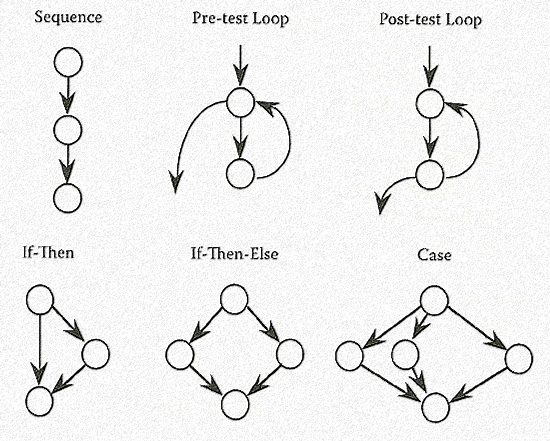
\includegraphics[scale=0.45]{CFG.png}
		\caption{Flow graph notation}
	\end{figure}

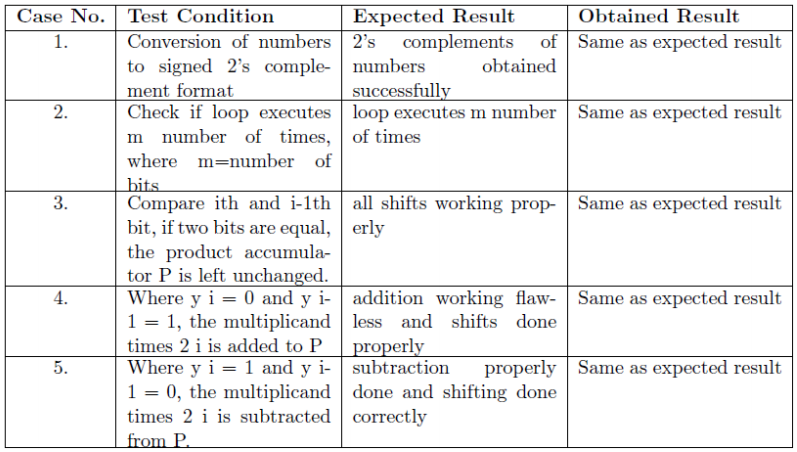
\includegraphics[width=\textwidth]{booth_whitebox}

\subsection{ POSITIVE/NEGATIVE TESTING }

\textbf{Positive Testing :}\\
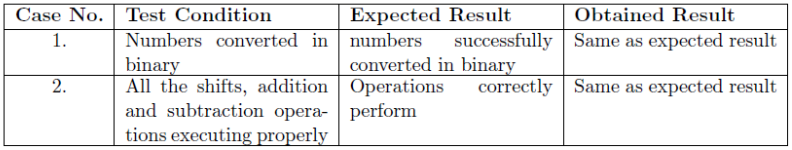
\includegraphics[width=\textwidth]{booth_positive}
\vspace{30px}

\textbf{Negative Testing :}\\
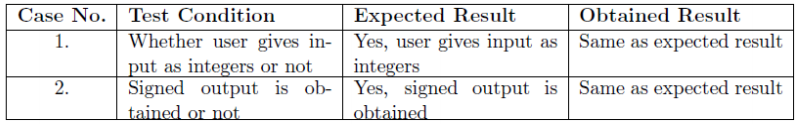
\includegraphics[width=\textwidth]{booth_negative}
\vspace{30px}

\section{Conclusion}
Thus we have studied Quick Sort and implemented it using parallel framework of Threads in java. We have also acquired an acute sense of syntheiszing the documentation of typical softwares created in the industry.

\end{document}